\section{Basic t-SNE Algorithm}
This section closely follows the Theoretical Foundations Paper \cite{JMLR:v23:21-0524} and \cite{vdMaa08} so far. 

Let $\{x_1, \dots , x_n \}$ with $x_i \in \mathbb{R}^d$ for all $1 \leq i \leq n$ be the a set of high-dimensional points we wish to visualize. We initialize a low-dimensional map $\{y_1, \dots , y_n\} \subset \mathbb{R}^2$ (Sometimes, a three-dimensional map is also considered. For the purpose of this thesis, we stick to two-dimensional maps). 

\subsection{Measuring High-Dimensional Similarities}

Instead of using the raw Euclidean distances between the high-dimensional data points, t-SNE measures pairwise similarities via probabilities. 
We define a joint probability distribution over all pairs of data points $\{(x_i, x_j)\}_{1 \leq i \neq j \leq n}$ via  
\begin{equation}
    p_{j|i} =  \frac{\exp(-\norm{x_i - x_j}_2^2 / 2\sigma_i^2)}{\sum_{k \in \{1,2, \dots, n\} \backslash \{i\}} \exp({-\norm{x_i - x_k}_2^2 / 2 \sigma_i^2})}
\end{equation}
which is then symmetrized to $p_{ij} = \frac{p_{i|j} + p_{j|i}}{2n}$. We set $p_{ii}=0$ for all $i$ since we are only interested in modelling pairwise similarities between points. In matrix form, we write $P = (p_{ij})_{1 \leq i, j \leq n}$. 
Large $p_{ij}$ values indicate that the points $x_i$ and $x_j$ closely resemble each other. 
Intuitively, one can think of $p_{j|i}$ as the probability that $x_i$ would choose $x_j$ as a neighbor if neighbors are chosen according to a Gaussian centered at $x_i$ with bandwidth $\sigma_i$. 

The bandwidths $\sigma_i$ of the Gaussian kernel can be adapted based on a fixed number called perplexity using binary search. See more on this in the section on perplexity. 

One might wonder why it is necessary to symmetrize the similarities. Just taking the $p_{j|i}$ leads to problems for outlier datapoints: since all pairwise distances $\norm{x_i - x_j}^2$ are large for an outlier datapoint $x_i$, all $p_{ij}$ values for this datapoint end up being very small. As a result, the location of the low-dimensional map point $y_i$ does not contribute very much to the loss function. With symmetrization, we ensure that $\sum_{j} p_{ij} > \frac{1}{2n}$ for all datapoints $x_i$. 

\subsection{Measuring Low-Dimensional Similarities}

We then also compute a similarity measure for points in the low-dimensional embedding as follows: 
\begin{equation}
    q_{ij} = \frac{(1+ \norm{y_i - y_j}_2^2)^{-1}}{\sum_{l, s \in \{1,2, \dots, n\}, l \neq s } (1+\norm{y_l - y_s}_2^2)^{-1}}
\end{equation}
where we again define $q_{ii} = 0$ for all $1 \leq i \leq n$. We can collect all of the points in a symmetrical matrix $Q = (q_{ij})_{1 \leq i, j \leq n}$. 

The central contribution of t-SNE over SNE is using the more heavy-tailed Student t-distribution instead of a Gaussian. 
This addresses the crowding problem, see \cite{vdMaa08}. 

\begin{figure}[h]
    \begin{center}
        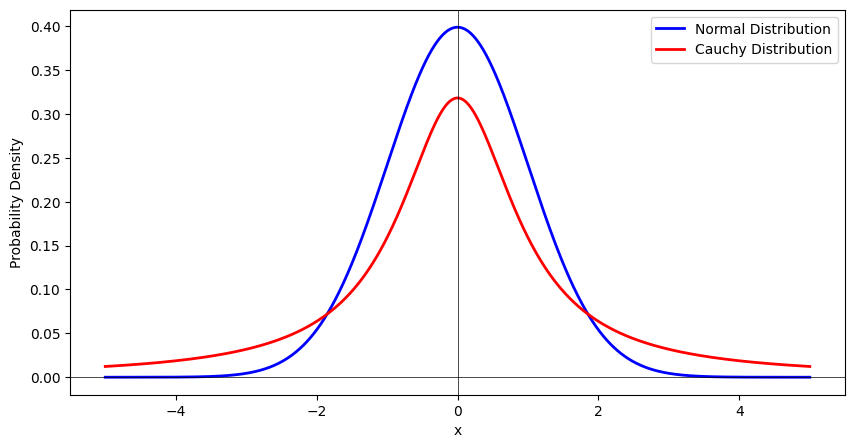
\includegraphics[width=0.9\linewidth]{Gaussian_Cauchy.png}
    \end{center}
\end{figure}

\subsection{The Loss Function}
The goal of the algorithm is now to get the similarities $P$ and $Q$ to be as close to each other as possible. 
A common choice for measuring the distance between two distributions is the Kullback-Leibler divergence. 

\begin{defi}[Kullback-Leibler Divergence]
    The \emph{Kullback-Leibler divergence} between two probability distributions $P$ and $Q$ over the same probability space is defined as:
    \[
    D_{\text{KL}}(P \parallel Q) = \sum_{x \in \mathcal{X}} P(x) \log\frac{P(x)}{Q(x)}
    \]
    for discrete distributions where \(\mathcal{X}\) is the domain of the distributions.
\end{defi}

The t-SNE algorithm now aims to find a low-dimensional representation $\mathcal{Y} = (y_1, \dots, y_n)$ that minimizes the KL-divergence between the similarity matrices $P$ and $Q$. We thus define the following loss function: 
\begin{equation}
    C(\mathcal{Y}) = D_{\text{KL}}(P \parallel Q) = \sum_{i,j \in \{1,\dots,n\}, i \neq j} p_{ij} \log \frac{p_{ij}}{q_{ij}}
\end{equation}
which leads to the following optimization problem: 
\begin{equation}
    (y_1, \dots y_n) = \argmin_{y_1, \dots y_n} C(\mathcal{Y}) = \argmin_{y_1, \dots y_n} \sum_{i,j \in \{1,\dots,n\}, i \neq j} p_{ij} \log \frac{p_{ij}}{q_{ij}}.
\end{equation}


Note that the Kullback-Leibler divergence is in fact not a metric, since it is not symmetric. 
One can observe that a large $p_{ij}$ being modeled by a small $q_{ij}$ leads to a bigger summand than using a large $q_{ij}$ to model a small $p_{ij}$. 
This means that our loss function places a large cost on using far-apart points to model points that are close in the original dataset. 
On the other hand, there is only a small cost to model points that are actually far apart as nearby in the embedding. 
This shows that we can expect a bigger focus on the preservation of local structure and is important to keep in mind when interpreting t-SNE embeddings, see \cite{Wa16Distill}. 

\subsection{Gradient Descent to Minimize Loss}
Minimizing the cost function can be achieved using a standard gradient-descent type algorithm, with an updating equation of 
\begin{equation}
    y_i^{(k+1)} = y_i^{(k)} + h \frac{\partial C}{\partial y_i}^{(k)} + m^{(k+1)}(y_i^{(k)} - y_i^{(k-1)}) 
\end{equation}
for $i=1,\dots,n$, where $h >0$ is a prespecified step size parameter, $m^{(k)} > 0$ is a momentum parameter and we denote the gradient of our loss function (with respect to $y_i$) as: 
\begin{equation}
    \frac{\partial C}{\partial y_i}^{(k)} = 4 \sum_{1 \leq j \leq n, j \neq i} (y_j^{(k)} - y_i^{(k)}) S_{ij}^{(k)} \in \mathbb{R}^2 \text{ with } S_{ij}^{(k)} = \frac{p_{ij} - q_{ij}^{(k)}}{1+ \norm{y_i^{(k)}-y_j^{(k)}}_2^2 } \in \mathbb{R}
\end{equation}
